\section{Auswertung}
\label{sec:Auswertung}

Die Ergebnisse der Messung der Verschiebung $D$ des Leuchtflecks in Abhängigkeit von der Beschleunigungsspannung $U_B$ und der Verschiebungsspannung $U_D$ sind in \autoref{tab:verschiebung} aufgelistet.

\begin{table}
    \centering
    \caption{Messergebnisse der Verschiebung $D$ des Leuchtflecks bei unterschiedlichen Beschleunigungsspannungen $U_B$ in Abhängigkeit der Verschiebungsspannung $U_D$, wobei $\SI{1}{Kästchen}=\SI{0.25}{Zoll}=\SI{0.635}{\centi\metre}$ ist.}
    \begin{tabular}{S S S S S S S}
        \toprule
        \multicolumn{2}{c}{\tableSI{U_B}{\volt}:} & {250} & {300} & {350} & {400} & {450} \\
        \midrule
        \tableSI{D}{Kästchen} & \tableSI{D}{\centi\metre} & \multicolumn{5}{c}{\tableSI{U_D}{\volt}} \\
        \midrule
        1 & 0.635 & 0.3 & 0.1 & 0.1 & 0.1 & 0.1 \\
        0 & 0.000 & 2.9 & 3.2 & 3.3 & 3.9 & 4.4 \\
        -1 & -0.635 & 6.4 & 8.2 & 8.9 & 10.3 & 11.9 \\
        -2 & -1.270 & 10.2 & 12.3 & 14.3 & 17.6 & 20.2 \\
        -3 & -1.905 & 13.3 & 17.0 & 20.5 & 24.6 & 28.2 \\
        -4 & -2.540 & 17.0 & 21.8 & 27.2 & 31.8 & 36.2 \\
        \bottomrule
    \end{tabular}
    \label{tab:verschiebung}
\end{table}

Die verschiedenen Messreihen sind in \autoref{fig:plot_verschiebung} dargestellt. 

\begin{figure}
    \centering
    \includegraphics[width=\textwidth]{build/plot_verschiebung.pdf}
    \caption{Plot der Messwerte aus \autoref{tab:verschiebung} mit entsprechenden Ausgleichsgeraden der Parameter aus \autoref{tab:ausgleichsrechnung}}
    \label{fig:plot_verschiebung}
\end{figure}

Die entsprechende Ausgleichsgerade wird nach \autoref{eq:verschiebung} über
\begin{equation}
    D(U_D) = a \cdot U_D + b
\end{equation}
mit der Funktion curve\_fit aus der Python Bibliothek SciPy berechnet.
Hier ist anzumerken, dass die ersten Messpunkte ($D=\SI{1}{Kästchen}$) sehr ungenau sind und nicht zum berechnen der Ausgleichsgerade verwendet werden.
Damit ergeben sich die in \autoref{tab:ausgleichsrechnung} aufgelisteten Parameter $a$ und $b$.

\begin{table}
    \centering
    \caption{Parameter der durchgeführten Ausgleichsrechnung}
    \begin{tabular}{S[table-format=3.0] S[table-format=-1.4(4)] S[table-format=1.3(3)]}
        \toprule
        \tableSI{U_B}{\volt} & \tableSI{a}{\frac{\centi\metre}{\volt}} & \tableSI{b}{\centi\metre} \\
        \midrule
        250 & -0.1808+-0.0028 & 0.531+-0.032 \\
        300 & -0.1379+-0.0022 & 0.454+-0.031 \\
        350 & -0.1067+-0.0028 & 0.313+-0.047 \\
        400 & -0.0905+-0.0011 & 0.327+-0.022 \\
        450 & -0.0795+-0.0006 & 0.333+-0.015 \\
        \bottomrule
    \end{tabular}
    \label{tab:ausgleichsrechnung}
\end{table}

Um nun die Empfindlichkeit des verwendeten Gerätes zu ermitteln, wird eine Ausgleichsrechnung der Parameter $a(U_B)$ über 
\begin{equation}
    a(U_B) = \frac{p_1}{U_B} + p_2
\end{equation} 
durchgeführt und ergibt
\begin{align*}
    p_1 &= \SI{-54+-3}{\centi\metre} = -E \\
    p_2 &= \SI{0.042+-0.008}{\frac{\centi\metre}} \, .
\end{align*}
Nach \autoref{eq:verschiebung} entpricht der berechnete Parameter $p_1$ betragsmäßig der sogenannten Empfindlichkeit $E = \frac{p L}{2 d}$.

\begin{figure}
    \centering
    \includegraphics[width=\textwidth]{build/plot_empfindlichkeit.pdf}
    \caption{Plot der Parameter $a$ aus \autoref{tab:ausgleichsrechnung} gegen die reziproke Beschleunigungsspannung $1/U_B$.}
    \label{fig:plot_empfindlichkeit}
\end{figure}

Ein Vergleichswert der Empfindlichkeit des benutzten Gerätes kann ermittelt werden, wenn diese über die Abmessungen des Gerätes aus \autoref{fig:abmessungen} berechnet wird.
Hier wurde die Y-Verschiebung gemessen, also ist
\begin{align*}
    p &= \SI{1.9}{\centi\metre} \\
    L &= \SI{14.3}{\centi\metre} \\
    d &= \SI{0.38}{\centi\metre} \, .
\end{align*}
Somit ergibt sich der Vergleichswert der Empfindlichkeit zu
\begin{equation*}
    E_\text{Vergleich} = \SI{35.75}{\centi\metre} \, .
\end{equation*}

\begin{figure}
    \centering
    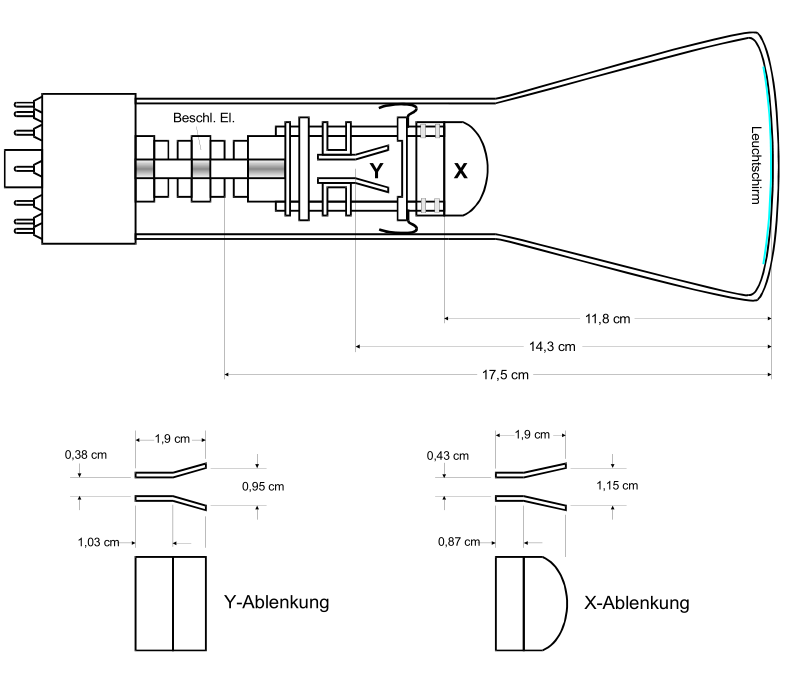
\includegraphics[width=0.7\textwidth]{images/bild5.png}
    \caption{Abmessungen der verwendeten Kathodenstrahlröhre.\cite{V501}}
    \label{fig:abmessungen}
\end{figure}



Die Untersuchung einer angelegten Sinusspannung an die X-Achse mit angelegter Sägezahnspannung an der Y-Achse ergab die Messergebnisse in \autoref{tab:frequenz}.
Die Messung der Höhe der Sinuskurve auf dem Leuchtschirm (peek-to-peek)
\begin{equation*}
    h\text{Sin} = \SI{1.27}{\centi\metre} \, .
\end{equation*}
Hier sei anzumerken, dass aufgrund eines fehlerhaften Gerätes diese Messwerte an einem anderen Gerät gemessen wurden.
Also wird im Folgenden für die Empfindlichkeit der Wert $E_\text{Vergleich}$ verwendet.

\begin{table}
    \centering
    \caption{Messergebnisse der Frequenz der Sägezahnspannung bei stehenden Bilder, also einem Frequenzverhältnis von $n \cdot \nu_\text{Säg} = \nu_\text{Sin}$}
    \begin{tabular}{S S}
        \toprule
        {n} & \tableSI{\nu_\text{Säg}}{\hertz} \\
        \midrule
        0.5 & 100.07 \\
        1.0 & 50.07 \\
        2.0 & 25.05 \\
        3.0 & 12.54 \\
        \bottomrule
    \end{tabular}
    \label{tab:frequenz}
\end{table}

Mithilfe dieser Messwerte kann also die Sinusfrequenz $\nu_\text{Sin} = n \cdot \nu_\text{Säg}$ gemittelt werden und ergibt
\begin{equation*}
    \nu_\text{Sin} = \SI{47+-3}{\hertz} \, .
\end{equation*}

Außerdem wird die Amplitude der Sinusspannung nach \autoref{eq:verschiebung} über
\begin{equation}
    U_\text{Sin} = \frac{1}{2} \cdot \frac{h_\text{Sin}}{E \cdot U_B}
\end{equation} 
mit $U_B = \SI{300}{\volt}$ zu 
\begin{equation*}
    U_\text{Sin} = \SI{5.329+-0.002}{\volt}
\end{equation*}
berechnet.

Vergleichswerte für die Sinusspannung und -frequenz wurden nicht gemessen.